\documentclass{article}

\usepackage{times}
\usepackage{uist}
%\usepackage[config, font=small, labelfont={sf,bf}, textfont=sf]{caption,subfig}
\usepackage[config, font=small, labelfont={sf,bf}, textfont=sf]{caption}
\usepackage{subfig}
\usepackage{graphicx}

\begin{document}

% --- Copyright notice ---
\conferenceinfo{UIST'11}{October 16-19, 2011, Santa Barbara, CA, USA}
\CopyrightYear{2011}
\crdata{978-1-4503-0716-1/11/10}

% Uncomment the following line to hide the copyright notice
\toappear{}
% ------------------------

\bibliographystyle{plain}

\title{Sketch It, Make It: Freehand Drawing for Precision Rapid Fabrication}

\author{
\parbox[t]{9cm}{\centering
	     {\em Author One}\\
	     Institution Name\\
             City, ST, USA\\
	     user@institution.net}
\parbox[t]{9cm}{\centering
	     {\em Author Two}\\
	     Institution Name\\
             City, ST, USA\\
	     user@institution.net}
}

\maketitle

% TODO: change this
\abstract Abstract goes here. 

\classification{I.3.5 [Computational Geometry and Object Modeling]: Modeling packages}

% TODO: change this
\terms{Design, Human Factors}

\keywords{sketching, rapid fabrication, design tools, constraints}

\tolerance=400 % prevent words from sticking out in the margin

%% \begin{figure}[tb]
%% \vspace{1.9in}
%% \caption{A figure caption.  It is set in 9 point Helvetica type, with a
%% 0.5 cm wider margin on both left and right sides.} 
%% \label{fig-example}
%% \end{figure}

\section{INTRODUCTION}

A growing community of self-described \textit{makers} design and build
many kinds of physical things~\cite{gershenfeld-fab}. Some are
electronic or robotic gizmos, while others are made from traditional
material. These ``new makers''~\cite{gross-new-makers} are empowered
by rapid fabrication machines like 3D printers and laser cutters.

It is possible that we are beginning to see a shift from an economy
based on mass-production (in factories) to one that includes
mass-customization (in homes, schools, and community
centers)~\cite{economist-fab}. Rapid fabrication machines continue to
decline in price while improving in quality. A new sector of
businesses use rapid fabrication to cater to the needs of hobbyist
designers as well as people that need highly customized
goods~\cite{nyt-rapidfab}.  For example, companies such as Ponoko
fabricate and send users physical output based on digital models
uploaded over the web.

Laser cutters are among the more popular rapid fabrication
machines. They can be thought of as a very fast, strong, and precise
automated razor blade, cutting through flat material (paper, wood,
plastic, metal, etc.) from directly above. Many items can be made
entirely with a laser cutter, aside from the occasional screw or glue.
Figure~\ref{fig:laser-example} shows several examples of useful items
made with laser cutters.

\begin{figure}[h]
\centering 
\subfloat[] {
  \label{fig:laser-example-a} 
  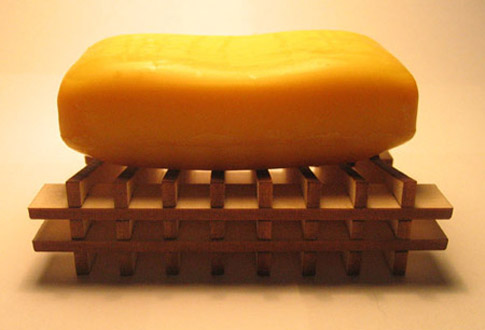
\includegraphics[width=0.4\linewidth]{img/flat-b.jpg}
}
\subfloat[] {
    \label{fig:laser-example-b}
    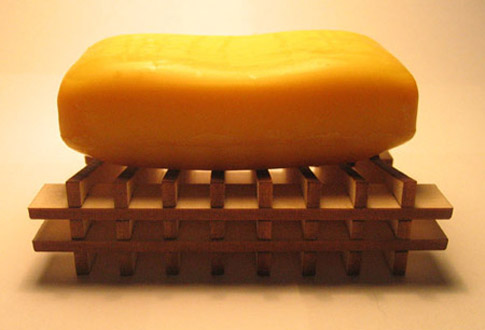
\includegraphics[width=0.4\linewidth]{img/flat-b.jpg}
}
\caption{Laser cut items.}
\label{fig:laser-example}
\end{figure}

Today, designers can choose among several modeling tools for laser
cutter projects. Adobe Illustrator, a general-purpose vector graphics
editor, is the most commonly used tool. Illustrator is full-featured
and has an interface new users find familiar. However, participants in
a formative study had a hard time using Illustrator quickly and
effectively when designing for laser cutters. Specialized CAD tools
like Rhino or SolidWorks are perhaps more appropriate for this kind of
modeling but they also have a substantial learning curve. If rapid
fabrication is to become common, appropriate modeling tools must be
made accessible to ordinary users~\cite{lipson-homefactory}.

Laser cut items are composed of parts cut from solid, flat pieces of
material. The primary concern of the designer is to define the path
taken by the laser cutter. Parts may be put together in various ways.
Pieces can be glued or screwed together in layers. Alternately the
user can design joints so the parts fit together. Most joints have
small margins of error. It is important that lengths, angles, and
relative position be indicated with precision for the parts to fit
together as they should.

In this paper, we present a modeling tool called ``Sketch It, Make
It'' (SIMI).  It is based on recognizing short sequences of sketched
input with a stylus. By using freehand drawn input, SIMI enables the
designer to iteratively and incrementally create laser cut models that
fit precise specifications.

We are inspired by the potential of freehand drawing as a basis for
our tool for several reasons. Sketching is quick and can be easily
learned. The technology is simple.  Unlike structured editing
software, a designer does not need to set the pencil's mode to line,
circle, or anything else. A freehand sketch can provide enough
information that others can translate it into a digital model. 

The primary contribution of this work is a system that embodies a new
way of designing precise 2D shapes by incremental sketch recognition
and rectification.

\section{RELATED WORK}

While ``the design process'' has important differences between
domains, there are two common properties to nearly all design
efforts. First, designers sketch throughout the process, particularly
in the beginning. Second, a computer tool is used to formalize the
design. This is confirmed by observations of graphic
designers~\cite{wong-rr-prototypes}, automotive
engineers~\cite{kara-styling}, and software
developers~\cite{dekel-improvised-notation}. Freehand drawing is a
powerful means for thinking and specifying design intent, but it is
disconnected from the computer aided portion of the design
process~\cite{company-sketching-in-engineering}. 

Computer support for fabrication design has been a topic of interest
for several decades, alternately called computer aided design (CAD) or
computer aided manufacturing (CAM). Sutherland's SketchPad
system~\cite{sutherland-sketchpad} is among the earliest and most
influential examples of interactive design software. SketchPad users
controlled the system by setting modes and parameters with one hand
and drawing on the screen with a light pen in the other. This form of
input enabled people to create mechanical parts that conformed to
engineering requirements. 

More recently, novel interfaces have been developed that enable users
to model items for fabrication by sketching. For example,
Plushie~\cite{mori-plushie} lets people design soft objects like
stuffed animals. Users create 3D models of bulbous objects by
sketching in a manner similar to Teddy~\cite{igarashi-teddy}. The
program creates a set of 2D shapes that users can cut from fabric,
sew, and fill with stuffing. 

Sketch Chair is a more recent example of a tool that helps make design
for rapid fabrication more accessible~\cite{saul-sketch-chair}. It
lets users sketch the contours of a chair's seat and back rest, and
using a different drawing mode, add legs. The system includes a
sophisticated physical simulator to let the designer explore its
physicality (for example to determine if it will remain upright). It
also allows designers to change subtle properties of curves using
on-screen control handles.

ParSketch~\cite{naya-parsketch} enables designers to create parametric
2D models by incrementally recognizing sketched geometry and
commands. It uses pressure to distinguish between linework (high
pressure) and constraint commands (lower pressure).

\section{FORMATIVE STUDY}

To better understand the domain of laser cutter fabrication we
conducted two related empirical studies. We analyzed laser-cut items
on community web sites to find common features. We also interviewed
people with experience designing these artifacts, and watched how they
worked. 

\subsection{Artifact Analysis}

Ponoko and Thingiverse are two popular web sites for selling or
sharing items that can be made with rapid fabrication like laser
cutters and 3D printers. We selected 55 laser-cut projects and
examined their attributes to better understand what people are really
making with laser cutters. The results of this analysis are shown in
Figure~\ref{fig:ponoko}.

\begin{figure}[h]
  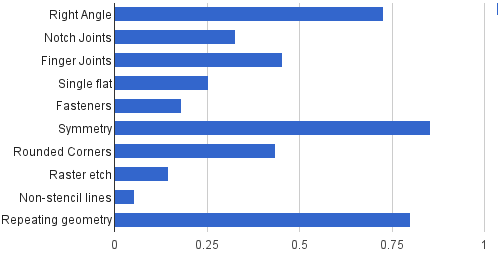
\includegraphics[width=0.9\linewidth]{img/ponoko-analysis.png}
  \caption{Frequency of certain attributes were present in laser-cut
    projects from Ponoko and Thingiverse.}
  \label{fig:ponoko}
\end{figure}

We used a set of ten properties to characterize each project. These
were chosen based on our own experience with items made with laser
cutters, as well as from observations from the formative study
discussed shortly. These properties are:

\begin{itemize}
\item \textit{Right Angle}: Dominant edges meet at 90-degree angles.
\item \textit{Notch and Finger Joints}: Two parts come together using one of
  the joints illustrated in Figure~\ref{fig:joint}.
\item \textit{Single part}: Project is composed of a single, flat piece of
  material (e.g. a coaster).
\item \textit{Fasteners}: Clear use of glue, screws, or bolts.
\item \textit{Symmetry}: Radial or linear symmetry is a dominant feature.
\item \textit{Rounded Corners}: Right-angle corners are slightly blunt.
\item \textit{Raster etch}: Laser cutter etched patterns (e.g. words,
  images) rather than cutting through material.
\item \textit{Non-stencil lines}: Instances where thin lines were cut.
\item \textit{Repeating geometry}: Linework is repeated several times.
\end{itemize}

\begin{figure}[h]
\centering 
\subfloat[Notch joints.] {
  \label{fig:joint-notch} 
  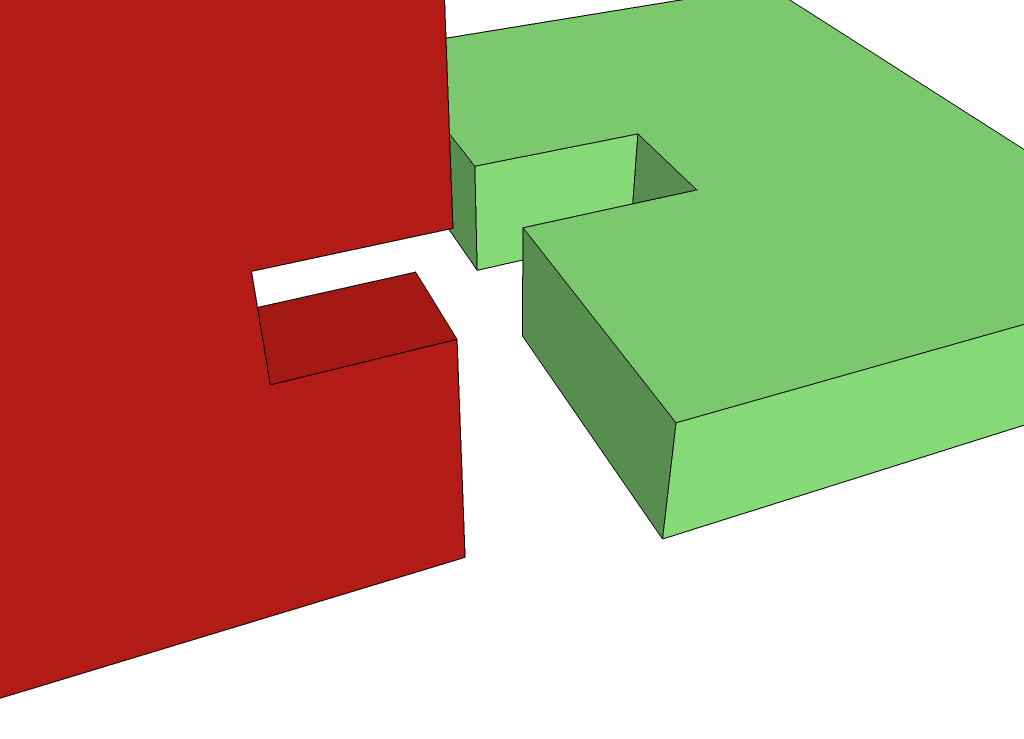
\includegraphics[width=0.4\linewidth]{img/joint-notch.png}
}
\subfloat[Finger joints, alternately called box joints.] {
    \label{fig:joint-finger}
    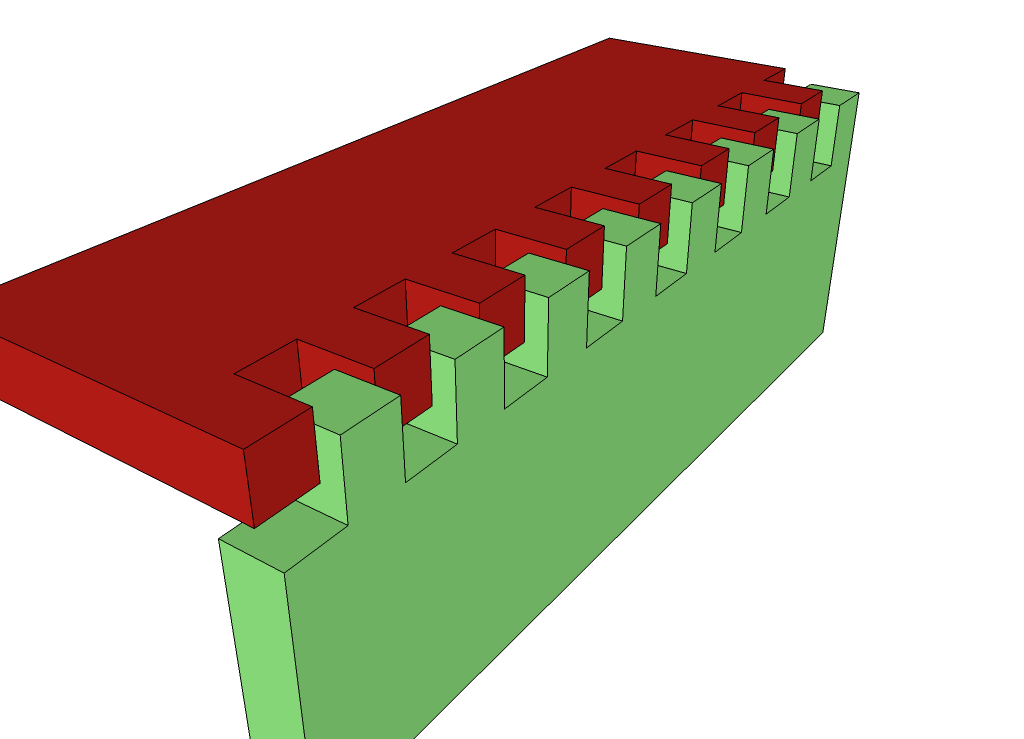
\includegraphics[width=0.4\linewidth]{img/joint-finger.png}
}
\caption{Two common joint types.}
\label{fig:joint}
\end{figure}

The purpose of single part projects were typically artistic, using
expressive, curvy linework. Among those objects composed of more than
one piece, nearly all used finger or notch joints
(Fig.~\ref{fig:joint}). The rest used fasteners.

The more professional-looking models were generally the ones that used
rounded corners. Raster etching was also used for artistic effect in
several cases. ``Non-stencil lines'' are thin lines cut all the way
through material. They can be used for artistic effect (e.g. to allow
light through). When used on flexible material they allow the part to
stretch differently.

Repeating geometry was found in most models (joints were excluded from
consideration). These patterns involve sequences of lines or curves
with consistent length and angles. Some patterns were quite ornate.

\subsection{Formative Study}
\label{sec:formative}

We interviewed designers to find out more about their work practices
and to better understand how they use their tools. The participants
have substantially different backgrounds: all have training in some
form of design, including mechanical engineering, graphic design, and
architecture. Each participant was asked to describe their design
process, and to show sketches or videos of their work. While there are
subtle (and some substantial) differences in their process, each
followed the following pattern.

They begin by thinking about a problem and making drawings by
hand. Some sketches are made to think about how to frame the project
(what it is for), while others help reason about how to make it (how
it works, how it fits together). Some designers explicitly noted that
sketching is a necessary part of the process; it would not be possible
to move forward without making freehand drawings. When the idea is
reasonably well-formed they will implement the model with a software
tool. It is common for this to involve translating a hand-made sketch
to a computer model (Figure~\ref{fig:translate}).

\begin{figure}[h]
  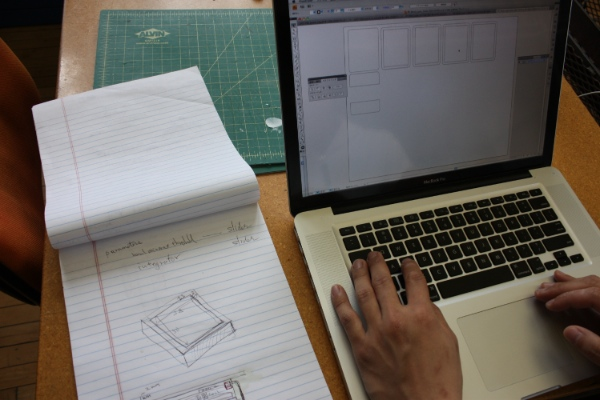
\includegraphics[width=0.9\linewidth]{img/translate-sketch-to-computer.jpg}
  \caption{A common part of desgining for laser cutters: translating a
    hand-made sketch to a computer modelling tool. The sketch includes
    a perspective drawing of the desired result, and 2D diagrams of
    individual parts with important dimensions indicated.}
  \label{fig:translate}
\end{figure}

Following the work practices interview, participants were asked to
implement the sketch shown in Figure~\ref{fig:interview-sketch} using
their software tool of choice. The purpose of this was to learn what
problems people encountered when executing the common task of
translating a sketch to a computer model. Each session lasted
approximately an hour and was split evenly between the interview and
implementation portions.

\begin{figure}[h]
\centering 
\subfloat[The part users set out to replicate.] {
  \label{fig:interview-sketch-1} 
  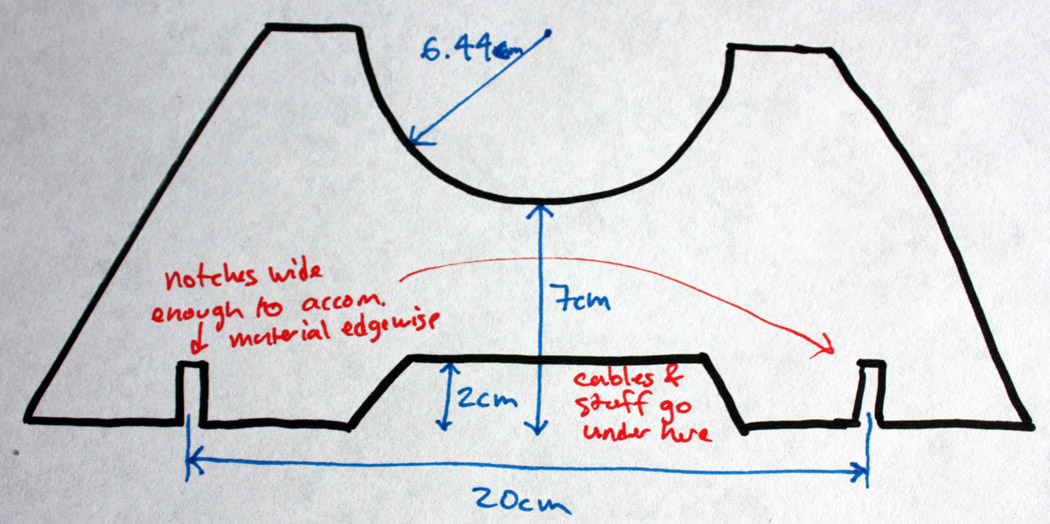
\includegraphics[width=0.9\linewidth]{img/laser-me-1.jpg}
}

\subfloat[Drawing of how the part is used in context.] {
    \label{fig:interview-sketch-2}
    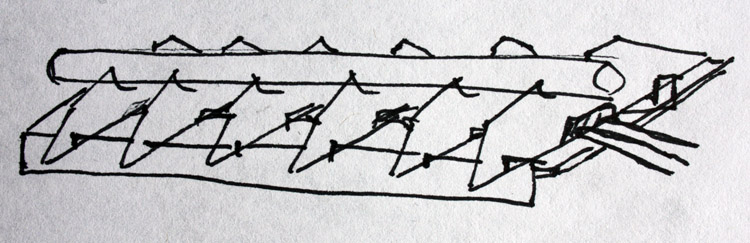
\includegraphics[width=0.9\linewidth]{img/laser-me-2.jpg}
}
\caption{Participants were asked to implement the stencil at the top
  using modeling software.}
\label{fig:interview-sketch}
\end{figure}

Participants mostly chose to implement the sketch with Illustrator (5
users), while another chose Rhino. In all cases, a designer's strategy
involved common activities: creating or editing boundaries, aligning
or snapping items, using guide lines or reference points, measuring
distances, specifying or changing lengths and angles, and creating
finished ``cut files'' that will be sent to the laser cutter. These
tasks are in addition to selecting/deselecting onscreen elements, or
viewport management like zooming and panning.

Participants in this experiment spent a good deal of time on operating
overhead. This includes (1) trying to find the appropriate tool for
the next task, (2) recovering from errors made when the wrong tool was
selected, or (3) when the tool behavior was inconsistent with the
user's intention. Approximately 50\% of the designer's time was spent
in this way.

For example, one user was aware of Illustrator's ``Path Finder'' tool
and wanted to use it. The user searched the program's menu structure
and slowly hovered over toolbar buttons to read tool tips before
finding it. Next, the designer invoked various functions of the Path
Finder, using the keyboard shortcut to undo after each attempt, as he
searched for the correct mode within the subcommand palette. This
process lasted approximately 80 seconds before finally being able to
continue.

Occasionally participants used features in rather strange ways to
achieve a desired outcome. In order to remove an unwanted segment of a
polyline, one participant (a graphic designer) chose to create an
opaque white rectangle to obscure it, rather than erase it. (``Don't
tell anyone I did this'', he said at the time). 

Similar episodes are common: a person \textit{should} know the
`correct' action, but takes an alternate approach. The alternative
might achieve the intended effect, but it might be less efficient
(more operations, longer execution time) or it might introduce
unwanted complexity (such as the invisible white rectangle).

To summarize, these are the common tasks and problems found during
this interview study:

\begin{itemize}
\item creating/editing boundaries
\item aligning/snapping items
\item using guide lines or reference points
\item measuring distances
\item specifying lengths/angles
\item creating cut files
\item selecting/deselecting
\item viewport management
\item finding and entering tool modes
\item recover from error (tool or user error)
\item `correct' action is unknown or hard to do
\end{itemize}

\section{SKETCH IT, MAKE IT}

Based on observation of designer work practices and the artifacts they
make, we have developed \textit{Sketch It, Make It} (SIMI), a
sketch-based tool for modeling laser cut items. We aim to address many
of the problems with currrent modeling systems enumerated above while
giving people a tool that specifically supports designing laser-cut
items.

% * map problems from earlier (x y z) to solutions in simi

% * overview of interaction

SIMI users draw with a stylus and can use an offhand button for a few
actions. The system recognizes input as either geometric linework or
gestural commands. Linework includes straight lines, elliptical arcs,
splines, circles, and ellipses. 

Users can issue commands on linework by drawing gestures. Some
gestures are recognized and acted on immediately, such as the erase
(scribble) gesture. Others, such as commands to constrain segments be
the same length, are recognized after the user presses the button, or
after a timeout.

When the user makes a closed 2D path, the system recognizes it as a
stencil. Stencils are shapes that can be placed on the virtual laser
cutter plane. Several copies of a stencil can be added. The system
generates a vector file that can be sent to a laser cutter without
modification.

After laser cutting the stencils, the user can assemble them to their
final configuration. Several examples of projects made with SIMI are
shown in Figure~\ref{fig:laser-example}.

\subsection{Implementation}

%* Stylus with offhand button

The guiding principle we used when developing SIMI is that the
designer should never need to set down their pen. Most input is
provided entirely with a stylus. A single button used by the
non-dominant hand gives access to additional commands.

* Gestures:

  - Latch (3 kinds) 

  - Erase 

  - undo/redo

  - right angle

  - same-length 

  - flow-selection

  - guide points

  - select stencils

* Constraints

  - introduce what they are

  - list types supported: right angle, same length, co-terminate, specific length

  - visual appearance

* Stencils (with or without holes)

\section{EVALUATION}

* screenshots/photos from user study

* other results from user study...

\section{ACKNOWLEDGMENTS}

% TODO: fill this in later. Leave left blank for blind review.

\bibliography{simi}

\end{document}
